\chapter{Chemical kinetics}
\label{ch:kinetics}

Thermodynamics tells us the destination; kinetics tells us the speed and the route. Flames exist
only because the route is fast at high temperature and almost blocked at room temperature.
A stoichiometric \ce{H_2}/air mixture can sit in a balloon for years, yet burns in microseconds once
a spark has made some radicals.

\section{Global versus elementary reactions}

The overall reaction $\ce{H_2}+\tfrac12\ce{O_2}\to\ce{H_2O}$ never happens as written: three
molecules would have to collide in exactly the right way and rearrange four bonds at once. What
happens instead is a network of \textbf{elementary reactions}, each a single collision event,
mostly involving highly reactive fragments called \textbf{radicals} (species with an unpaired
electron: H, O, OH, \ce{HO_2}).

\begin{intuition}
A global reaction is like a train timetable that lists only ``London $\to$ Edinburgh''. Elementary
reactions are the individual stations and connections. If you want to know what happens when a
station closes (extinction), when the train sets off (ignition) or how fast it travels (flame
speed), you need the full route.
\end{intuition}

\section{Why reactions need energy: collision theory}
\label{sec:collision}

\begin{figure}[H]
\centering
\begin{tikzpicture}[xscale=1.4,yscale=1.1]
  \draw[->] (0,0) -- (7.2,0) node[below left] {reaction coordinate};
  \draw[->] (0,0) -- (0,4.4) node[above] {energy};
  \draw[very thick,intu] plot[smooth] coordinates {(0.3,1.8) (1.4,1.8) (2.6,2.6) (3.5,3.8) (4.4,2.4) (5.6,0.8) (6.8,0.8)};
  \node[lbl] at (0.9,2.15) {reactants};
  \node[lbl] at (6.2,1.15) {products};
  \node[lbl,align=center] at (3.5,4.25) {transition state};
  \draw[<->,hot,thick] (1.2,1.8) -- (1.2,3.8) node[midway,left] {$E_a$};
  \draw[dashed] (1.2,3.8) -- (3.5,3.8);
  \draw[<->,keyc,thick] (6.4,1.8) -- (6.4,0.8) node[midway,right] {$\Delta h_R<0$};
  \draw[dashed] (1.4,1.8) -- (6.6,1.8);
  \draw[<->,warn,thick] (5.0,0.8) -- (5.0,3.8) node[midway,right] {$E_a-\Delta h_R$ (reverse)};
\end{tikzpicture}
\caption{Energy along the reaction path. Even an exothermic reaction must first climb a barrier
$E_a$. The reverse reaction must climb $E_a+|\Delta h_R|$, which is why exothermic reactions are
effectively one-way at low temperature.}
\label{fig:barrier}
\end{figure}

\begin{derivation}[Arrhenius law from collisions]
Consider $\mathrm A+\mathrm B\to$ products. Treat molecules as hard spheres with collision
cross-section $\sigma_{AB}=\pi(r_A+r_B)^2$. A molecule A moving at relative speed $\bar c_{rel}$
sweeps a volume $\sigma_{AB}\bar c_{rel}$ per second and hits every B in it. Kinetic theory gives
$\bar c_{rel}=\sqrt{8k_BT/(\pi m_{AB})}$, with reduced mass $m_{AB}=m_Am_B/(m_A+m_B)$. Collisions per
unit volume per second:
\[
Z_{AB}=\sigma_{AB}\,\bar c_{rel}\;n_An_B .
\]
Only collisions whose energy along the line of centres exceeds $E_a$ react. From the Maxwell--Boltzmann
distribution that fraction is $e^{-E_a/\Ru T}$. Add a ``steric factor'' $P\le1$ for the orientation.
The reaction rate in kmol/m$^3$/s is then $k\,[\mathrm A][\mathrm B]$ with
\begin{equation}
  k(T)=\underbrace{P\,\sigma_{AB}\sqrt{\frac{8k_BT}{\pi m_{AB}}}\,N_A}_{\propto T^{1/2}}\,
  e^{-E_a/\Ru T}.
\end{equation}
Generalising the $T^{1/2}$ to $T^\beta$ (to absorb effects the hard-sphere model misses) gives the
\textbf{modified Arrhenius} form used in every mechanism file:
\begin{equation}
  \boxed{k(T)=A\,T^{\beta}\exp\!\left(-\frac{E_a}{\Ru T}\right)}
  \label{eq:arrhenius}
\end{equation}
\end{derivation}
\begin{symbols}
$r_A$, $r_B$ & molecular radii & \si{\metre}\\
$\sigma_{AB}$ & collision cross-section $\pi(r_A+r_B)^2$ & \si{\metre\squared}\\
$\bar c_{rel}$ & mean relative speed of A and B & \si{\metre\per\second}\\
$m_{AB}$ & reduced mass $m_Am_B/(m_A+m_B)$ & \si{\kilo\gram}\\
$n_A$, $n_B$ & number densities & \si{\per\metre\cubed}\\
$Z_{AB}$ & collision rate per unit volume & \si{\per\metre\cubed\per\second}\\
$E_a$ & activation energy (barrier height) & \si{\joule\per\kilo\mole}\\
$P$ & steric (orientation) factor & \nodim\\
$k_B$, $N_A$ & Boltzmann constant, Avogadro's number & \si{\joule\per\kelvin}, \si{\per\kilo\mole}\\
$k(T)$ & rate constant; for a bimolecular reaction & \si{\metre\cubed\per\kilo\mole\per\second}\\
$A$ & pre-exponential factor (order $n$ reaction) & $(\si{\metre\cubed\per\kilo\mole})^{n-1}\si{\per\second}\,\si{\kelvin}^{-\beta}$\\
$\beta$ & temperature exponent & \nodim\\
$[\mathrm A]$, $[\mathrm B]$ & molar concentrations & \si{\kilo\mole\per\metre\cubed}\\
\end{symbols}

\begin{intuition}
$A T^\beta$ counts how often molecules meet in the right orientation; it varies slowly with $T$.
$e^{-E_a/\Ru T}$ is the fraction that meet hard enough; it varies violently. Radical--radical
recombinations have $E_a\approx 0$: every encounter works, and they are fast at any $T$.
Reactions that break a strong bond (like $\ce{H}+\ce{O_2}\to\ce{O}+\ce{OH}$,
$E_a\approx\SI{70}{\kilo\joule\per\mole}$) need high temperatures.
\end{intuition}

\paragraph{Units of $A$.} For a reaction of overall order $n$ (number of reactant molecules,
including third bodies), $k$ has units $(\si{\metre\cubed\per\kilo\mole})^{n-1}\,\si{\per\second}$.
Mechanism files often use cm, mol, cal. Cantera converts on load, but be careful when copying
numbers by hand.

\section{Law of mass action and production rates}
\label{sec:massaction}

Write reaction $i$ as $\sum_k\nu'_{ki}\mathcal M_k\rightleftharpoons\sum_k\nu''_{ki}\mathcal M_k$. The
collision argument generalises: the rate is proportional to the product of reactant concentrations,
each raised to its stoichiometric coefficient. The \textbf{rate of progress} is
\begin{equation}
  q_i=k_{f,i}\prod_kC_k^{\nu'_{ki}}-k_{r,i}\prod_kC_k^{\nu''_{ki}}
  \qquad[\si{\kilo\mole\per\metre\cubed\per\second}],
\end{equation}
and the \textbf{net molar production rate} of species $k$ sums over all reactions:
\begin{equation}
  \wdot_k=\sum_{i=1}^{I}\nu_{ki}\,q_i,\qquad \nu_{ki}=\nu''_{ki}-\nu'_{ki}.
  \label{eq:wdot}
\end{equation}

\begin{symbols}
$q_i$ & net rate of progress of reaction $i$ & \si{\kilo\mole\per\metre\cubed\per\second}\\
$k_{f,i}$, $k_{r,i}$ & forward, reverse rate constants & depend on order\\
$C_k$ & molar concentration & \si{\kilo\mole\per\metre\cubed}\\
$\nu'_{ki}$, $\nu''_{ki}$, $\nu_{ki}$ & reactant, product, net stoichiometric coefficients & \nodim\\
$\wdot_k$ & net molar production rate of $k$ & \si{\kilo\mole\per\metre\cubed\per\second}\\
$W_k\wdot_k$ & net mass production rate of $k$ & \si{\kilo\gram\per\metre\cubed\per\second}\\
$I$, $K$ & number of reactions, of species & \nodim\\
\end{symbols}
In matrix form $\bm{\wdot}=\mathsf N\bm q$, with $\mathsf N$ the $K\times I$ stoichiometric matrix.
The mass production rate is $W_k\wdot_k$ [\si{\kilo\gram\per\metre\cubed\per\second}]. Mass is
conserved in every reaction, so $\sum_kW_k\wdot_k=0$ exactly.

\begin{lstlisting}
gas.forward_rate_constants    # k_f,i
gas.net_rates_of_progress     # q_i          [kmol/m^3/s]
gas.net_production_rates      # omega_dot_k  [kmol/m^3/s]
gas.heat_release_rate         # -sum_k h_k omega_dot_k  [W/m^3]
\end{lstlisting}

\section{Reverse rates come from thermodynamics}
\label{sec:reverse}

\begin{derivation}[detailed balance]
At equilibrium every elementary reaction is individually balanced: $q_i=0$. Therefore
\[
\frac{k_{f,i}}{k_{r,i}}=\prod_kC_{k,\rm eq}^{\nu_{ki}}\equiv K_{c,i}(T).
\]
Using $C_k=X_kp/(\Ru T)$ and \eqref{eq:KX}:
\begin{equation}
  K_{c,i}=K_{p,i}\left(\frac{p^\circ}{\Ru T}\right)^{\Delta\nu_i},\qquad
  K_{p,i}=\exp\!\left(-\frac{\Delta G_i^\circ}{\Ru T}\right).
\end{equation}
Mechanisms therefore list only $(A,\beta,E_a)$ for the forward direction. Cantera computes
$k_{r,i}=k_{f,i}/K_{c,i}$ from the NASA polynomials. This guarantees that a kinetic simulation
run for long enough ends exactly at the thermodynamic equilibrium of \chapref{ch:equilibrium}.
\end{derivation}
\begin{symbols}
$k_{f,i}$, $k_{r,i}$ & forward, reverse rate constants of reaction $i$ & depend on reaction order\\
$C_{k,\rm eq}$ & equilibrium concentration of species $k$ & \si{\kilo\mole\per\metre\cubed}\\
$K_{c,i}$ & concentration-based equilibrium constant & $(\si{\kilo\mole\per\metre\cubed})^{\Delta\nu_i}$\\
$K_{p,i}$ & pressure-based equilibrium constant & \nodim\\
$\Delta\nu_i$ & net change in moles in reaction $i$ & \nodim\\
$\Delta G_i^\circ$ & standard Gibbs energy change of reaction $i$ & \si{\joule\per\kilo\mole}\\
$p^\circ$, $\Ru$, $T$ & standard pressure, gas constant, temperature & \si{\pascal}, \si{\joule\per\kilo\mole\per\kelvin}, \si{\kelvin}\\
\end{symbols}

\section{Third bodies and pressure dependence}

Recombination such as $\ce{H}+\ce{OH}\to\ce{H_2O}$ releases a lot of energy into the new bond. If
nothing removes it, the molecule flies apart again. A \textbf{third body} M (any molecule) must
collide at the same time and carry the energy away:
\[
\ce{H}+\ce{OH}+\mathrm M\to\ce{H_2O}+\mathrm M,\qquad
q=k\,[\ce{H}][\ce{OH}][\mathrm M],\qquad [\mathrm M]=\sum_k\epsilon_kC_k .
\]

\begin{symbols}
$[\mathrm M]$ & effective third-body concentration & \si{\kilo\mole\per\metre\cubed}\\
$\epsilon_k$ & collision efficiency of species $k$ & \nodim\\
$k$ & termolecular rate constant & \si{\metre^6\per\kilo\mole\squared\per\second}\\
\end{symbols}
The \textbf{efficiencies} $\epsilon_k$ capture that some molecules absorb energy better: \ce{H_2O}
($\epsilon\approx 12$) is far better than Ar ($\epsilon\approx 0.7$).

\paragraph{Fall-off (Lindemann).} For reactions like $2\ce{OH}(+\mathrm M)\rightleftharpoons\ce{H_2O_2}(+\mathrm M)$ the
collision with M is only needed at low pressure. At high pressure the energised complex is
always stabilised and the rate stops depending on [M]:
\begin{equation}
  k=\frac{k_0[\mathrm M]\,k_\infty}{k_\infty+k_0[\mathrm M]}=k_\infty\frac{P_r}{1+P_r},\qquad P_r=\frac{k_0[\mathrm M]}{k_\infty},
\end{equation}

\begin{symbols}
$k_0$ & low-pressure limit rate constant & \si{\metre^6\per\kilo\mole\squared\per\second}\\
$k_\infty$ & high-pressure limit rate constant & \si{\metre\cubed\per\kilo\mole\per\second}\\
$P_r$ & reduced pressure & \nodim\\
$F$ & Troe broadening factor & \nodim\\
\end{symbols}
so $k\approx k_0[\mathrm M]$ at low $p$ and $k\approx k_\infty$ at high $p$. Troe's form multiplies
this by a broadening factor $F$. In the YAML file these appear as \code{type: falloff} with
\code{low-P-rate-constant}, \code{high-P-rate-constant} and \code{Troe:} entries.

\section{The hydrogen--oxygen chain}
\label{sec:h2chain}

The heart of all hydrogen combustion (and of the H/O sub-mechanism of every hydrocarbon) is:
\begin{center}
\begin{tabular}{lll}
\toprule
& reaction & role \\
\midrule
R1 & $\ce{H_2}+\ce{O_2}\to\ce{HO_2}+\ce{H}$ & \textbf{initiation}: makes the first radicals (slow, high $E_a$) \\
R2 & $\ce{H}+\ce{O_2}\rightleftharpoons\ce{O}+\ce{OH}$ & \textbf{chain branching}: 1 radical $\to$ 2 \\
R3 & $\ce{O}+\ce{H_2}\rightleftharpoons\ce{H}+\ce{OH}$ & \textbf{chain branching}: 1 radical $\to$ 2 \\
R4 & $\ce{OH}+\ce{H_2}\rightleftharpoons\ce{H_2O}+\ce{H}$ & \textbf{chain propagation}: 1 radical $\to$ 1, makes \ce{H_2O} \\
R5 & $\ce{H}+\ce{O_2}+\mathrm M\rightleftharpoons\ce{HO_2}+\mathrm M$ & \textbf{termination} (at low $T$, high $p$): reactive H $\to$ sluggish \ce{HO_2} \\
R6 & $\ce{H}+\ce{OH}+\mathrm M\rightleftharpoons\ce{H_2O}+\mathrm M$ & \textbf{termination / recombination}: releases most of the heat \\
\bottomrule
\end{tabular}
\end{center}

\begin{figure}[H]
\centering
\begin{tikzpicture}[node distance=14mm and 18mm,
  sp/.style={circle,draw,thick,minimum size=11mm,font=\small,fill=#1!15},
  sp/.default=hot]
  \node[sp=gray] (H2O2) {$\ce{H_2},\ce{O_2}$};
  \node[sp,right=of H2O2] (H) {H};
  \node[sp,above right=of H] (O) {O};
  \node[sp,below right=of H] (OH) {OH};
  \node[sp=keyc,right=28mm of OH] (H2O) {\ce{H_2O}};
  \node[sp=cold,below=of H] (HO2) {\ce{HO_2}};
  \draw[->,thick] (H2O2) -- node[above,lbl] {R1} (H);
  \draw[->,very thick,hot] (H) -- node[above left,lbl] {R2 (+\ce{O_2})} (O);
  \draw[->,very thick,hot] (H) -- node[above right,lbl,pos=0.5] {R2} (OH);
  \draw[->,very thick,hot] (O) to[bend left=25] node[above right,lbl] {R3 (+\ce{H_2}): H + OH} (OH);
  \draw[->,very thick,hot] (O) to[bend right=50] node[above,lbl] {R3} (H);
  \draw[->,thick,keyc] (OH) -- node[below,lbl] {R4 (+\ce{H_2})} (H2O);
  \draw[->,thick,keyc] (OH) to[bend left=40] (H);
  \draw[->,thick,cold] (H) -- node[left,lbl] {R5 (+\ce{O_2}+M)} (HO2);
  \draw[->,thick,keyc,dashed] (OH) to[bend left=45] node[above,lbl] {R6 (+H+M)} (H2O);
\end{tikzpicture}
\caption{The \ce{H_2}/\ce{O_2} chain. Red arrows multiply radicals (branching), green convert
radicals into product while keeping the chain alive (R4 also hands the H atom back, curved green arrow), blue removes the active H atom into the much
less reactive \ce{HO_2}.}
\label{fig:chain}
\end{figure}

\begin{derivation}[net effect of one branching cycle]
Add R2 + R3 + 2$\times$R4:
\[
\ce{H}+\ce{O_2}+3\,\ce{H_2}\;\to\;2\,\ce{H_2O}+3\,\ce{H}.
\]
One H atom goes in, \textbf{three} come out. Each cycle multiplies the radical pool, and the
radical population grows exponentially. This is chain branching.
\end{derivation}
\begin{symbols}
H, O & hydrogen and oxygen atoms (radicals) & --\\
OH & hydroxyl radical & --\\
\ce{HO_2} & hydroperoxyl radical (much less reactive than H) & --\\
R2, R3, R4 & reactions of the table above (branching, branching, propagation) & --\\
\end{symbols}

\begin{derivation}[branching versus termination: the crossover temperature]
Let $n$ be the H-atom concentration and focus on its two fates: R2 (rate $k_2[\ce{O_2}]n$), which
via the cycle above returns net $+2$ radicals, and R5 (rate $k_5[\mathrm M][\ce{O_2}]n$), which
removes it. Then
\begin{equation}
  \od{n}{t}\approx \dot r_{\rm init}+\big(2k_2-k_5[\mathrm M]\big)[\ce{O_2}]\,n .
\end{equation}
If $2k_2>k_5[\mathrm M]$ the coefficient is positive and $n$ grows like $e^{t/\tau}$: \textbf{explosion}.
If it is negative, $n$ settles at a small steady value: \textbf{no explosion}. The boundary
$2k_2(T)=k_5(T)[\mathrm M]$ is the \textbf{crossover temperature}. $k_2$ has a large activation energy and
$k_5$ has none, so branching wins at high $T$. $[\mathrm M]=p/\Ru T$, so termination gains with
pressure.
\end{derivation}
\begin{symbols}
$n$ & concentration of H atoms & \si{\kilo\mole\per\metre\cubed}\\
$\dot r_{\rm init}$ & rate at which initiation creates radicals & \si{\kilo\mole\per\metre\cubed\per\second}\\
$k_2$ & rate constant of R2 (bimolecular) & \si{\metre\cubed\per\kilo\mole\per\second}\\
$k_5$ & rate constant of R5 (termolecular) & \si{\metre^6\per\kilo\mole\squared\per\second}\\
$[\mathrm M]$, $[\ce{O_2}]$ & third-body and oxygen concentrations; $[\mathrm M]\approx p/\Ru T$ & \si{\kilo\mole\per\metre\cubed}\\
$(2k_2-k_5[\mathrm M])[\ce{O_2}]$ & net radical growth rate $=1/\tau$ & \si{\per\second}\\
\end{symbols}

\begin{figure}[H]
\centering
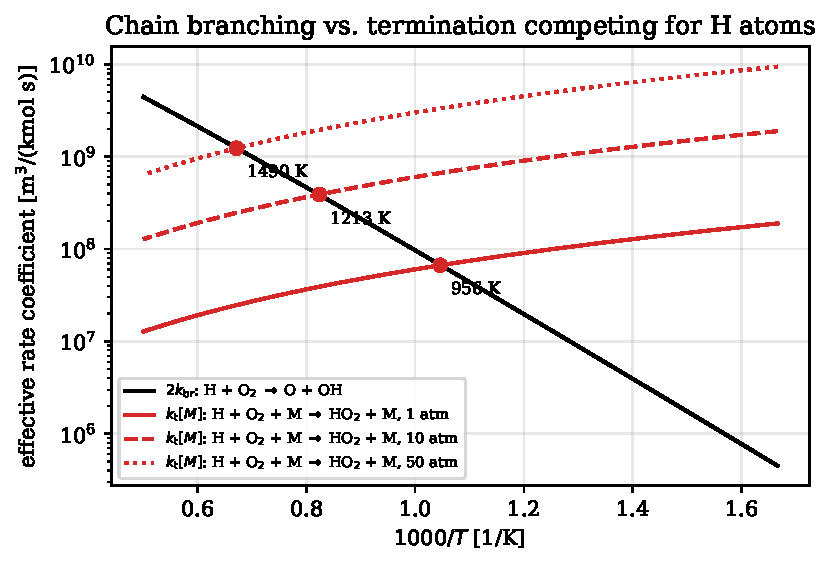
\includegraphics[width=0.85\textwidth]{arrhenius_crossover}
\caption{Arrhenius plot computed from \code{h2o2.yaml}. The branching line (black) is steep (large
$E_a$). The termination lines (red) are almost flat and move up with pressure. Their intersections
are the crossover temperatures: about \SI{950}{\kelvin} at 1 atm, rising with $p$. Below
crossover, hydrogen chemistry is ``slow''; above it, ``explosive''.}
\label{fig:arrh}
\end{figure}

\begin{intuition}
This single competition explains a surprising amount:
\begin{itemize}
  \item Why mixtures need $T\gtrsim\SI{1000}{\kelvin}$ to burn vigorously, which matters for
        flammability limits (Project Part~1, Task~1).
  \item Why ignition delay has a kink as a function of temperature (\figref{fig:taudelay}).
  \item Why hydrogen flame speeds \emph{decrease} with pressure: higher $[\mathrm M]$ favours R5 over R2
        (Project Part~3, Task~5).
  \item Why a flame can be extinguished: if strain or heat loss lowers the reaction-zone
        temperature towards crossover, branching collapses (Project Part~2).
\end{itemize}
\end{intuition}

\section{Heat release}

Most of the heat is \emph{not} released in the branching steps (R2 is endothermic!) but in the
recombination and propagation steps that form \ce{H_2O} (R4, R6). The local volumetric
\textbf{heat release rate} is
\begin{equation}
  \dot q=-\sum_k\hat h_k(T)\,\wdot_k\qquad[\si{\watt\per\metre\cubed}],
\end{equation}

\begin{symbols}
$\dot q$ & volumetric heat release rate & \si{\watt\per\metre\cubed}\\
$\hat h_k$ & molar enthalpy of $k$ (including formation) & \si{\joule\per\kilo\mole}\\
$\wdot_k$ & net molar production rate & \si{\kilo\mole\per\metre\cubed\per\second}\\
\end{symbols}
because destroying a species of enthalpy $\hat h_k$ and making another of lower enthalpy frees
the difference as sensible heat.

\section{Stiffness of chemistry}

Each species has a characteristic time scale $\tau_k\sim C_k/|\wdot_k|$. Radicals live for
nanoseconds; \ce{NO} forms over milliseconds to seconds. Formally the time scales are the
inverse eigenvalues of the chemical Jacobian $\partial\bm{\wdot}/\partial\bm C$, and they span 8--10
orders of magnitude. This is the stiffness of \secref{sec:stiff}. It is why Cantera uses
implicit integrators and why you never want to write your own explicit chemistry loop.

\section{Mechanism files}

A mechanism is a list of species (with thermo and transport data) plus a list of reactions (with
Arrhenius parameters). \code{h2o2.yaml} has 10 species and 29 reactions; GRI-Mech 3.0
(\code{gri30.yaml}) has 53 species and 325 reactions for natural gas. The anatomy of the YAML format is
shown in \secref{sec:ct-yaml}.

\begin{warning}
A mechanism is a \emph{model}, validated over a range of $T$, $p$, $\phi$ against experiments
(ignition delays, flame speeds). Outside that range it can be wrong. GRI-Mech~3.0 was
designed for natural gas, not hydrogen. For \ce{H_2} use a dedicated H/O mechanism
(\code{h2o2.yaml}, or literature mechanisms by Li et al., Burke et al., \'O~Conaire et al.).
\end{warning}

\section{Global one-step reactions (for scaling arguments)}
\label{sec:global}

For back-of-envelope reasoning we sometimes pretend the whole chain is one step:
\begin{equation}
  \wdot_F=-A\,[F]^a[O]^b\,e^{-E/\Ru T},\qquad n=a+b\ \text{(overall order)} .
\end{equation}

\begin{symbols}
$[F]$, $[O]$ & fuel, oxidiser concentrations & \si{\kilo\mole\per\metre\cubed}\\
$a$, $b$, $n$ & reaction orders in fuel, oxidiser, overall & \nodim\\
$A$ & pre-factor & $(\si{\metre\cubed\per\kilo\mole})^{n-1}\si{\per\second}$\\
$E$ & global activation energy & \si{\joule\per\kilo\mole}\\
\end{symbols}
Since $[F]=\rho Y_F/W_F\propto p$, the mass reaction rate scales like $p^{n}$ at fixed $T$ and
composition. We will use this in \chapref{ch:premixed} to predict how flame speed depends on
pressure. The \emph{effective} order of \ce{H_2}/air chemistry is less than 2 near crossover, precisely
because the termination step R5 gains with pressure.

\begin{selfcheck}
\begin{enumerate}
  \item R2 is endothermic. Why is it nevertheless the most important reaction in hydrogen combustion?
  \item Why does the recombination R6 become faster at high pressure, and why does that move heat
        release closer to the reaction zone?
  \item Using \figref{fig:arrh}, estimate the crossover temperature at 10 atm. What does it imply
        for ignition at engine-like pressures?
\end{enumerate}
\end{selfcheck}
